
%*******************************************************************************
%*********************************** First Chapter *****************************
%*******************************************************************************
%!TEX root = 0.main.tex

\section{Improving Deep Sphere}
\subsection{Adapting Belkin's setting to HEALPix sampling}

Getting inspired from the work flow presented above, we try to replicate the first theorem obtained in \textbf{Towards a theoretical foundation of Laplacian-based manifold methods} but not in the case of random Laplacians, but in the case of deterministic ones where the sampling is given by the HEALPix scheme. This analysis will be a preparatory work to further studies, since as we pointed out so far, from this kind of convergence nothing is said about the convergence of eigenvalues and eigenvectors. However, this study could maybe tell us something about the equivariance of the graph with respect to the action of the rotation group $SO(3)$.


We remind that \textbf{in order to adapt this proof to our needs, we need to find an another inequality to substitute Hoeffding's inequality.}


\paragraph{Definitions}

$n$ defines the number of vertices in the graph, $N$ defines the parameter $N_{side}$
\begin{definition}{Graph Laplacian}
	$$ \left(\mathbf L_n^t\right)_{ij}=\begin{cases}
	-w_{ij}, & i\neq j\\
	\sum_{k}w_{ik}, & i=j
	\end{cases}$$
\end{definition}
\begin{definition}{Point cloud Laplace operator}
	$$L_n^t:\quad(L_n^tf)(y) = \frac{1}{n}\left[ \sum_{i=0}^{n-1} e^{-\frac{||x_i-y||^2}{4t}}\left(f(y)-f(x_i)\right)\right]$$
\end{definition}
\begin{definition}{Functional approximation to the Laplace-Beltrami operator} \label{eq: my L^t}
	$$L^t:\quad L^tf(y) := \int_{\mathcal S_2}e^{-\frac{||p-x||^2}{4t}}\left(f(y)-f(x)\right)d\mu(x)$$
\end{definition}


\subsubsection{Pointwise convergence of the Graph Laplacian in the HEALPix case}

Here we want to prove that 
$$\forall f \text{ Lipschiz,}\quad \forall y\in\mathcal S_2,  \quad\quad L_n^tf(y)\rightarrow \frac{1}{|\mathcal S_2|}\int e^{-\frac{||x-y||^2}{4t}}\left(f(y)-f(x)\right)d\mu(x) = \frac{1}{|\mathcal S_2|} L^tf(y)$$

This will be an easy but introductory result to the main result proved in Step 2.

\begin{proof}
	We know by construction that the HEALPix sampling cut the sphere into equal areas. Let us note the surface of one level $S_N$, and the maximum distance to the center point of one surface\textbf{ $d_{N}$}.
	Let us assume that the function $f$ is $L$ Lipschitz, we have
	\[
	\int_{\sigma_{i}}f({\bf x})\text{d}{\bf x}-\frac{1}{2}Ld_{N}S_{N}\leq S_{N}f({\bf x}_{i})\leq\int_{\sigma_{i}}f({\bf x})\text{d}{\bf x}+\frac{1}{2}Ld_{N}S_{N}.
	\]
	Hence we have:
	\[
	\sum_{i}\int_{\sigma_{i}}f({\bf x})\text{d}{\bf x}-\sum_{i}\frac{1}{2}Ld_{N}S_{N}\leq S_{N}\sum_{i}f({\bf x}_{i})\leq\sum_{i}\int_{\sigma_{i}}f({\bf x})\text{d}{\bf x}+\sum_{i}\frac{1}{2}Ld_{N}S_{N}
	\]
	and 
	\[
	\left|S_{N}\sum_{i}f({\bf x}_{i})-\int f({\bf x})\text{d}{\bf x}\right|\le\frac{1}{2}Ld_{N}S_{tot}
	\]
	where $S_{tot}$ is the the total surface of the sphere. Now we need to characterize $d_{N}$ with respect of $N$ and $L$ with respect of $m$ and $\ell$. 
	
	

	
	Thanks to this result, we have the following two point wise convergences
	
	$$\forall f \text{ Lipschiz,}\quad \forall y\in\mathcal S_2,  \quad\quad \frac{1}{n}\sum_i e^{-\frac{||x_i-y||^2}{4t}}\rightarrow \frac{1}{|\mathcal S_2|}\int e^{-\frac{||x-y||^2}{4t}}d\mu(x)$$
	$$\forall f \text{ Lipschiz,}\quad \forall y\in\mathcal S_2,  \quad\quad \frac{1}{n}\sum_i e^{-\frac{||x_i-y||^2}{4t}}f(x_i)\rightarrow \frac{1}{|\mathcal S_2|}\int e^{-\frac{||x-y||^2}{4t}}f(x)d\mu(x)$$
	
	Remembering the definition of the extension of the graph Laplacian we have the following point wise convergence:
	$$\forall f \text{ Lipschiz,}\quad \forall y\in\mathcal S_2,  \quad\quad L_n^tf(y)\rightarrow \frac{1}{|\mathcal S_2|}\int e^{-\frac{||x-y||^2}{4t}}\left(f(y)-f(x)\right)d\mu(x) = \frac{1}{|\mathcal S_2|} L^tf(y)$$
\end{proof}
\paragraph{Step 2: replacing Hoeffding's inequality}
\begin{figure}[h!]
	\label{fig:Belkin proof}
	\caption{Old proof we need to modify}
	\centering
	\fbox{\includegraphics[width=0.9\textwidth]{figs/literaturereview/oldproof.png}}
\end{figure}
In the previous paragraph we already proved that \textit{keeping t fixed} $L_n^tf(x)\rightarrow L^tf(x)$. We now want to prove the following thing:
$$\left|\frac{1}{4\pi t^2}\left(L_n^tf(x) - \frac{1}{|\mathcal S_2|}L^tf(x)\right)\right|\xrightarrow[n\to \infty]{t\to 0}0$$
\textit{for $t\to0$ and $n\to\infty$ at the same time}. In other words, we want to prove that there exists a sequence $(t_n), \lim_{n\to\infty}t_n=0$ such that 
$$\forall f \text{ Lipschitz, } \forall x\in\mathcal S_2 \quad \left|\frac{1}{4\pi t_n^2}\left(L_n^{t_n}f(x) -\frac{1}{|\mathcal S_2|} L^{t_n}f(x)\right)\right|\xrightarrow{n\to \infty}0$$

\begin{proof}
	
	We define for simplicity of notation
	$$\phi^t(x;y) := e^{-\frac{||x-y||^2}{4t}}\left(f(y)-f(x)\right)$$
	$$K^t(x,y) :=  e^{-\frac{||x-y||^2}{4t}}$$
	$$N := N_{side}$$
	
	we start by writing the following chain of inequalities
	$$||L_n^tf-\frac{1}{|\mathcal S_2|}L^tf||_\infty = \max _{y\in \mathcal S_2} \left|L_n^tf-\frac{1}{|\mathcal S_2|}L^tf\right|=$$
	$$= \max _{y\in \mathcal S_2} \left| \frac{1}{n} \sum_{i=1}^n \phi^t(x_i; y)-\frac{1}{|\mathcal S_2|} \int_{\mathcal S_2} \phi^t(x;y)d\mu(x) \right|$$
	$$\leq \max _{y\in \mathcal S_2} \sum_{i=1}^n  \left| \frac{1}{n}  \phi^t(x_i; y)-\frac{1}{|\mathcal S_2|} \int_{A_i} \phi^t(x;y)d\mu(x) \right|$$
	$$= \frac{1}{|\mathcal S_2|} \max _{y\in \mathcal S_2} \sum_{i=1}^n  \left| \frac{|\mathcal S_2|}{n}  \phi^t(x_i; y)-\int_{A_i} \phi^t(x;y)d\mu(x) \right|$$
	$$= \frac{1}{|\mathcal S_2|} \max _{y\in \mathcal S_2} \sum_{i=1}^n  \left| A_i  \phi^t(x_i; y)-\int_{A_i} \phi^t(x;y)d\mu(x) \right|$$
	$$\leq \frac{1}{|\mathcal S_2|} \max _{y\in \mathcal S_2} \left[ n \mathcal L_{\phi^t_y} \max_{i=1,...n} (d_i|A_i|)  \right]$$
	
	where $\mathcal L_{\phi^t_y}$ is the Lipschitz constant of $x \rightarrow \phi^t(x, y)$ and where we used for the last inequality the arguments used in Step 1. If we assume $\max_{i=1,...n} (d_i|A_i|) \leq \frac{C}{N^3}$ (meaning $\max_{i=1,...n} d_i \leq \frac{C}{\sqrt{n}}$ and $\max_{i=1,...n} |A_i| \leq \frac{C}{n}$)
	and remember that for HEALPix $n=12N^2$
	
	$$\leq \frac{1}{|\mathcal S_2|} \max _{y\in \mathcal S_2} \left[ 12 \mathcal L_{\phi^t_y} \frac{C}{N} \right]$$
	
	Let's now find the explicit dependence $t\rightarrow \mathcal L_{\phi^t_y}$
	
	$\mathcal L_{\phi^t_y} = ||\partial_x\phi^t(x;y)||_\infty = ||\partial_x\left(K^t(x;y)f(x)\right)||_\infty = ||\partial_x K^t(x;y)f(x) + K^t(x;y)\partial_x f(x)||_\infty \leq$
	
	$ \leq ||\partial_x K^t(x;y)f(x)||_\infty + ||K^t(x;y)\partial_x f(x)||_\infty \leq  ||\partial_x K^t(x;y)||_\infty||f(x)||_\infty + ||K^t(x;y)||_\infty||\partial_x f(x)||_\infty = $
	
	$ = ||\partial_x K^t(x;y)||_\infty||f(x)||_\infty + ||\partial_x f(x)||_\infty = \mathcal L_{K^t_y} ||f||_\infty + ||\partial_xf||_\infty = \mathcal L_{K^t_y} ||f||_\infty + \mathcal L_f$
	
	where $\mathcal L_{K^t_y}$ is the Lipschitz constant of $x\rightarrow K^t(x;y)$. We can observe that such constant does not depend on $y$. Thus
	
	$\mathcal L_{K^t_y} = \norm{\partial_x e^{-\frac{x^2}{4t}}}_\infty = \norm{\frac{x}{2t}e^{-\frac{x^2}{4t}}}_\infty = \left. \frac{x}{2t}e^{-\frac{x^2}{4t}}\right|_{x=\sqrt{2t}}=(2et)^{-\frac{1}{2}}\propto t ^ {-\frac{1}{2}}$
	
	So we can continue
	
	$$ \frac{1}{|\mathcal S_2|} \max _{y\in \mathcal S_2} \left[ 12 \mathcal L_{\phi^t_y} \frac{C}{N} \right]\leq$$
	$$ \leq \frac{1}{|\mathcal S_2|} \left[   \frac{12C}{N} \left( (2et)^{-\frac{1}{2}} \norm{f}_\infty + \mathcal L_f \right)\right]\leq$$
	$$  \leq \frac{1}{|\mathcal S_2|} \frac{12C\norm{f}_\infty}{N(2et)^\frac{1}{2}} +   \frac{1}{|\mathcal S_2|} \frac{12C}{N}\mathcal L_f$$
	
	So we have that, rescaling by a factor $\frac{1}{t}\frac{1}{(4\pi t)^{\frac{k}{2}}}$
	
	$$\left.\norm{\frac{1}{t}\frac{1}{(4\pi t)^{\frac{k}{2}}}\left(L_n^tf-\frac{1}{|\mathcal S_2|}L^tf\right)}_\infty\right|_{k=2}\leq$$
	$$\leq \frac{1}{4\pi t^2}\norm{\left(L_n^tf-\frac{1}{|\mathcal S_2|}L^tf\right)}_\infty \leq$$
	$$ \leq \frac{3C}{\pi |\mathcal S_2|}\left[\frac{\norm{f}}{\sqrt{2e}}\frac{1}{Nt^\frac{5}{2}} + \frac{\mathcal L_f}{Nt^2}\right]$$
	
	we want $\begin{cases}
	t \rightarrow 0\\
	N \rightarrow \infty\\
	Nt^\frac{5}{2} \rightarrow \infty\\
	Nt^2 \rightarrow \infty
	\end{cases}$ in order for $ \frac{3C}{\pi |\mathcal S_2|}\left[\frac{\norm{f}}{\sqrt{2e}}\frac{1}{Nt^\frac{5}{2}} + \frac{\mathcal L_f}{Nt^2}\right] \xrightarrow[t\to 0 ]{N\to\infty}0$
	
	This is true if $\begin{cases}
	t(N) = N^\beta, &\beta\in(-\frac{2}{5}, 0) \\
	t(N) = N^\beta, &\beta\in(-\frac{1}{2}, 0)
	\end{cases} \implies t(N) = N^\beta, \quad \beta\in(-\frac{2}{5}, 0)$
	
	Indeed 
	
	$Nt^\frac{5}{2}=N^{\frac{5}{2}\beta+1}\xrightarrow{N \to \infty} \infty$ since $\frac{5}{2}\beta+1>0 \iff \beta>-\frac{2}{5}$
	
	$Nt^2=N^{2\beta+1}\xrightarrow {N \to \infty} \infty$ since $2\beta+1>0 \iff \beta>-\frac{1}{2}$
	
	So, for $t=N^\beta$ with $\beta\in(-\frac{2}{5}, 0)$ we have that 
	
	$$\begin{cases}
	(t_N)\xrightarrow{N\to\infty}0\\
	\norm{\frac{1}{4\pi t_N^2}L_n^{t_N}f-\frac{1}{|\mathcal S_2|}\frac{1}{4\pi t_N^2}L^{t_N}f}_\infty  \xrightarrow{N\to\infty}0
	\end{cases}$$
	
	
	thanks to the fact that - proof in \cite{Belkin:2005:TTF:2138147.2138189} - 
	$$\frac{1}{4\pi t^2} L^tf(y) \xrightarrow{t\to 0 } \frac{1}{|\mathcal S_2|}\triangle_{\mathcal S_2}f(y)$$
	we conclude that
	$$\forall y\in\mathcal S_2 \quad \lim_{N\to\infty}\frac{1}{4\pi t_N^2} L_n^{t_N}f(y) =  \lim_{N\to\infty}\frac{1}{|\mathcal S_2|}\frac{1}{4\pi t_N^2} L^{t_N}f(y) = \frac{1}{|\mathcal S_2|^2}\triangle_{\mathcal S_2}f(y) $$
\end{proof}
We can see that the result obtained has the same form than the result obtained in \cite{Belkin:2005:TTF:2138147.2138189}. If Belkin et al. proved convergence in the random case for $\beta \in (-\frac{1}{4}, 0)$, we proved convergence in the HEALPix case for $\beta \in (-\frac{2}{5}, 0)$. This kind of result can be interpreted in the following way. In order to have convergence, we need to reduce the kernel width but \textit{not so fast} compared to the resolution of the graph. In other words, the kernel width has to be reduced but is somewhat limited by the resolution of the graph, that has to increase faster than $t^\frac{2}{5}$.
\subsection{How to build a better graph}
Current state of the art: DeepSphere.
Problems: we don't see the convergence expected. in figure \ref{fig:DeepSphere} we see that as $N_{side}$ grows, the eigenspaces of the graph Laplacian do not get more and more aligned with the eigenspaces spanned by the spherical harmonics, as we expected. Why? The parameters to choose are the following: the standard deviation of the Gaussian kernel $t$ and the number of neighbors of the graph. We'll see that the main cause of this bad behavior is the fixed number of neighbors used in \cite{DeepSphere} for the construction of the graph. We'll see that to obtain the desired convergence it is necessary to increase the number of neighbors as we decrease sigma, as we can show hereunder.
\begin{figure}[h]
	\label{fig:DeepSphere}
	\caption{Results from DeepSphere}
	\centering
	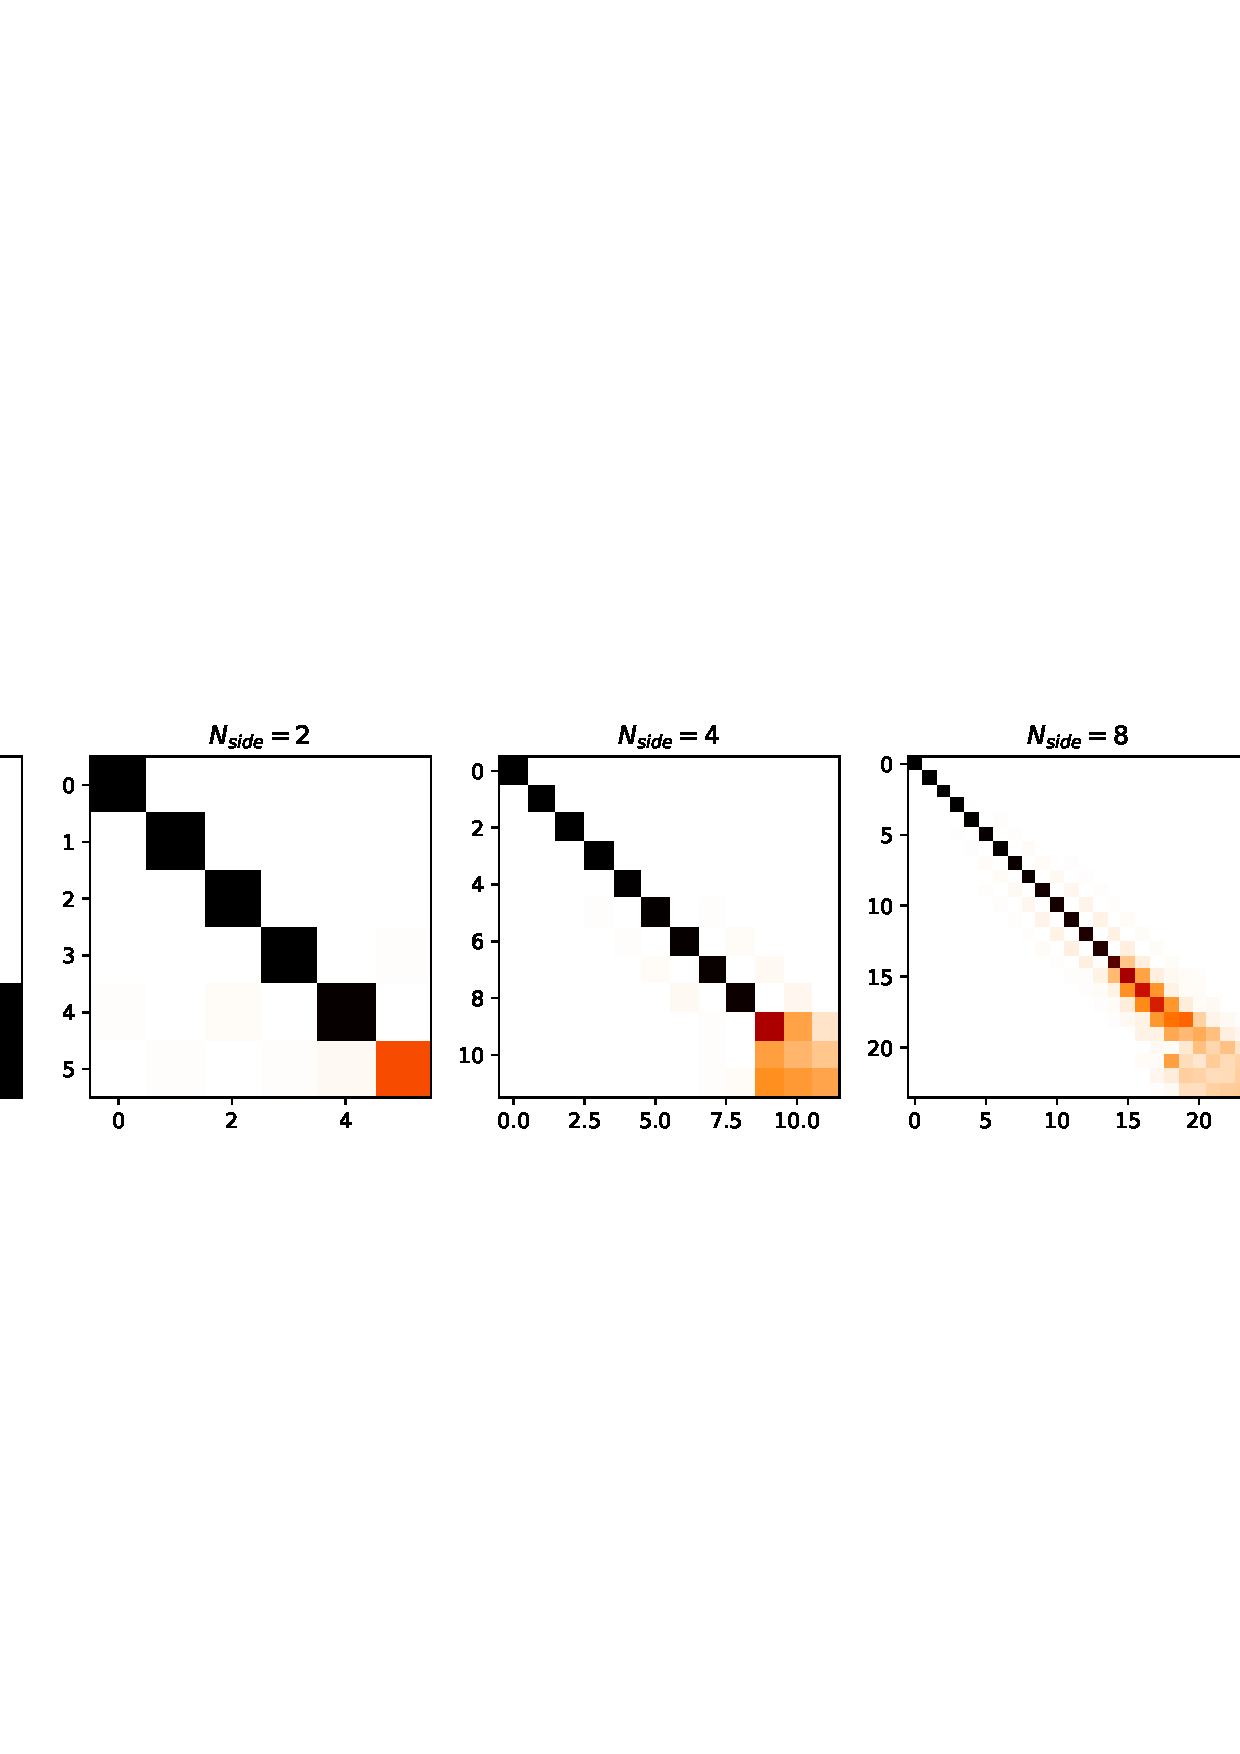
\includegraphics[width=0.9\textwidth]{../codes/02.HeatKernelGraphLaplacian/HEALPix/06_figures/deepsphere_original.png}
	\includegraphics[width=0.9\textwidth]{../codes/02.HeatKernelGraphLaplacian/HEALPix/06_figures/deepsphere_original_diagonal.png}	
\end{figure}
\subsubsection{About the kernel width $t$}
Intuition: with a big $t$, the kernel is very wide and the graph can not distinguish the high frequencies. In other words, if we build a radius graph with $d=\bar d$ and connect all the neighbors of a node with the same weights $w$, all the variations on those nodes are indistinguishable. thus, above a certain frequency where the variations reach a wavelength $\omega \leq \bar d$, any graph operator would be blind to such frequencies (indeed, any reordering of the signal on the neighbors would lead to the same result). Thus, if we want our graph Laplacian to be able to distinguish such frequencies, we need our weight to change significantly in a short radius, that means \textbf{setting a $t$ of the order of magnitude of the nearest neighbors of a node}. This intuition was already used in DeepSphere. 

Remember that the convergence result proved in the previous section is valid for a full graph: let's try to see how a full graph built with the same values of $t$ used in \cite{DeepSphere} behaves. 
In figure \ref{fig:DeepSphere_full} we see how for such a full graph it is indeed possible to observe the expected convergence:
\begin{figure}[h]
	\label{fig:DeepSphere_full}
	\caption{DeepSphere \textbf{full}}
	\centering
	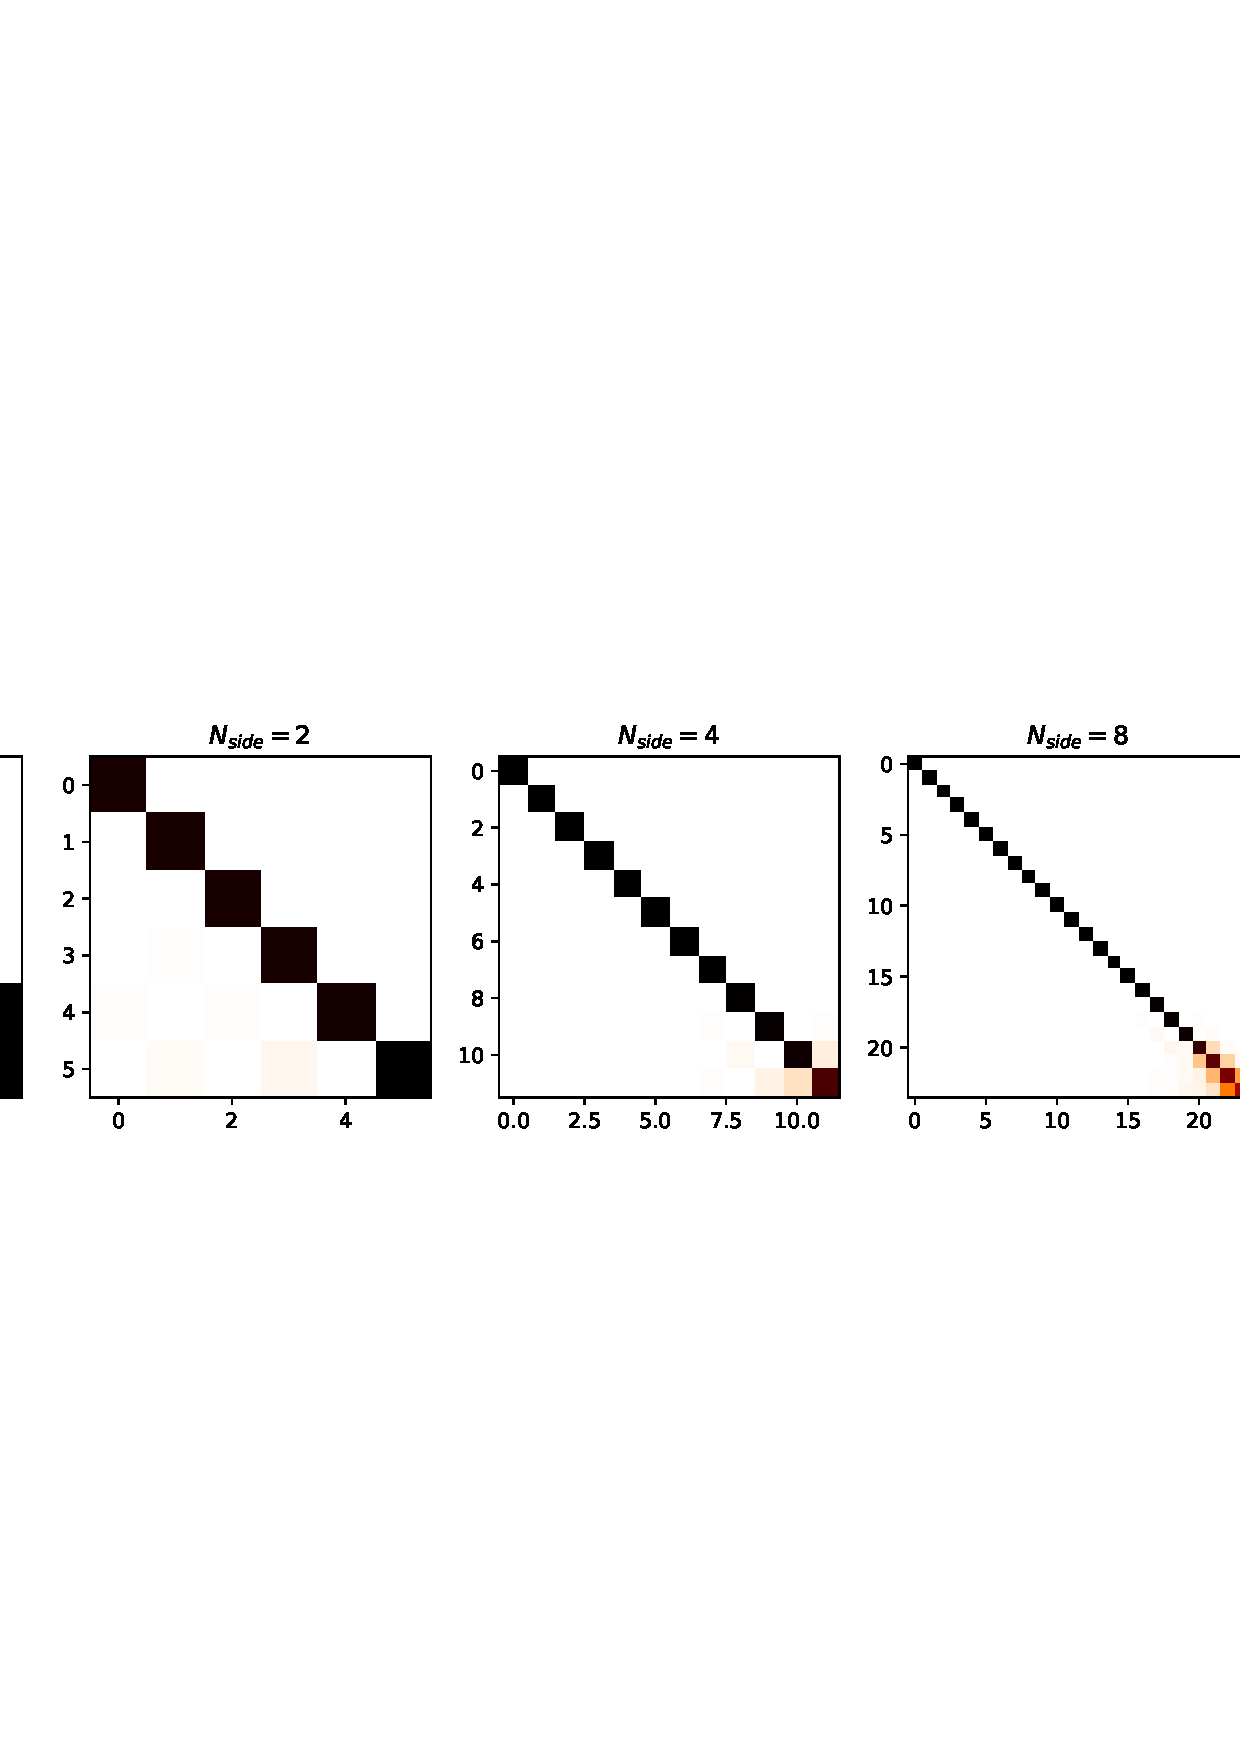
\includegraphics[width=0.9\textwidth]{../codes/02.HeatKernelGraphLaplacian/HEALPix/06_figures/deepsphere_full.png}
	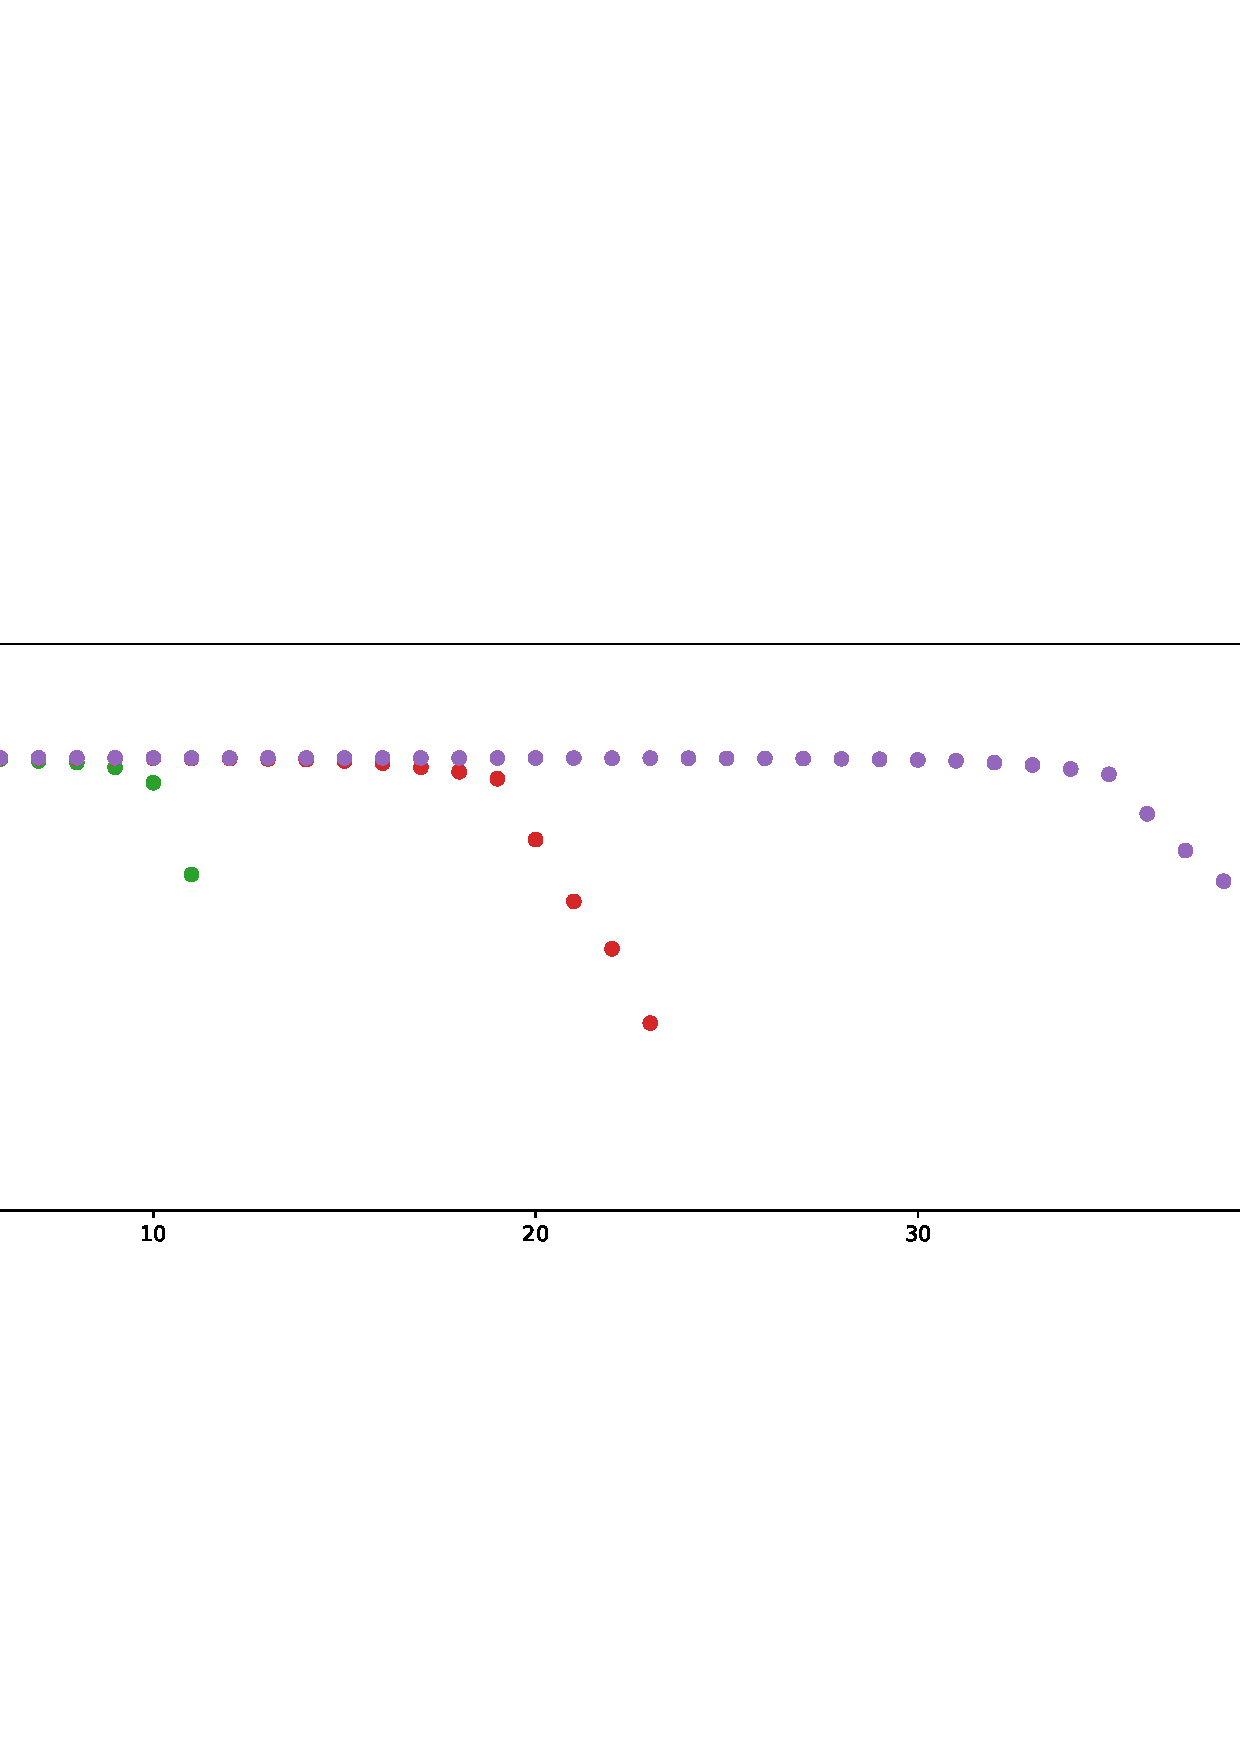
\includegraphics[width=0.9\textwidth]{../codes/02.HeatKernelGraphLaplacian/HEALPix/06_figures/deepsphere_full_diagonal.png}	
\end{figure}
A quick heuristic grid search has been used to find the following optimal parameters for different values of $N_{side}$ in the case of a full graph. The results are shown in figure \ref{fig:t}. We can see that the heuristic way of \cite{DeepSphere} of setting the standard deviation $t$ produces results very close to the optimal value.

\begin{figure}[h]
	\label{fig:t}
	\caption{Standard deviation of the Gaussian kernel  in a loglog plot. A straigh line indicates a polynomial relation.}
	\centering
	\includegraphics[width=0.5\textwidth]{../codes/02.HeatKernelGraphLaplacian/HEALPix/06_figures/kernelwidth.png}
\end{figure}

However, it is worth showing how the spectrum of the graph is sensible to such parameter. In figure \ref{fig:t_sensitity} it is shown how of the alignment of the eigenspaces is sensible to small changes of $t$. To produce this image $N_{side}$ was set to 16, and a full graph has been build where $t$ has been set first equal to the one used in \cite{DeepSphere} ($t=0.00647$) and then to the optimal value obtained in this work $t=0.015$.

\begin{figure}[h]
	\label{fig:t_sensitity}
	\caption{Standard deviation of the Gaussian kernel}
	\centering
	\includegraphics[width=0.9\textwidth]{../codes/02.HeatKernelGraphLaplacian/HEALPix/06_figures/t_sensitivity.png}
	\includegraphics[width=0.9\textwidth]{../codes/02.HeatKernelGraphLaplacian/HEALPix/06_figures/t_sensitivity_diagonal.png}
\end{figure}

\subsubsection{Reducing the number of neighbors}
For what it concerns how to make the graph sparse, the intuition is the following: remember that we want our graph Laplacian to approximate the operator $L^t$
$$\frac{1}{n}\left(\sum_i e^{-\frac{||x_i-y||^2}{4t}}(f(y)-f(x_i)) \right) \approx \frac{1}{ 4\pi}\int_\mathcal M e^{-\frac{||x-y||^2}{4t}}\left(f(y)-f(x)\right)d\mu(x) $$

However, with a full graph the operation of filtering with a polynomial of the graph Laplacian would cost $\mathcal O (n^2)$, same order of magnitude of the method proposed in \cite{bibid}. We want a method to make the graph sparse such that the number of non-null entries of the Laplacian is linear $\mathcal O (n)$, making the filtering operation $f\rightarrow \mathcal P(L)f$ linear in the number of pixels. Deferrard et al. \cite{bibid} fixed the number of neighbors to 7/8. However, their results do not show the expected spectral convergence.
Making the graph sparse means approximating some weights $w_{i,j}=e^{-\frac{||x_i-x_j||^2}{4t}} \approx 0$. For this to be accurate we need those weights to be close to 0. A method to be sure that the approximation isn't too bad is the following: \textbf{instead of fixing the number of neighbors, fixing a threshold $k$ on $w_{i,j}=e^{-\frac{||x_i-x_j||^2}{4t}}$ such that} 

$$w_{i,j} = \begin{cases}
e^{-\frac{||x_i-x_j||^2}{4t}}\quad& \text{if } e^{-\frac{||x_i-x_j||^2}{4t}} \geq k\\
0 \quad & \text{if } e^{-\frac{||x_i-x_j||^2}{4t}} < k
\end{cases}$$

By setting $k = 0.01$ here's the results:

\begin{center}
	\begin{tabular}{ c|c} 
		
		$N_{side}$ & Number of neighbors \\ 
		
		1 & 11 \\ 
		2 & 16 \\ 
		4 & 37 \\ 
		8 & 43 \\ 
		16 & 52 \\ 
		
	\end{tabular}
\end{center}

\begin{figure}[h]
	\label{fig:DeepSphere_thresholded}
	\caption{Deepsphere \textbf{thresholded at $k=0.01$}}
	\centering
	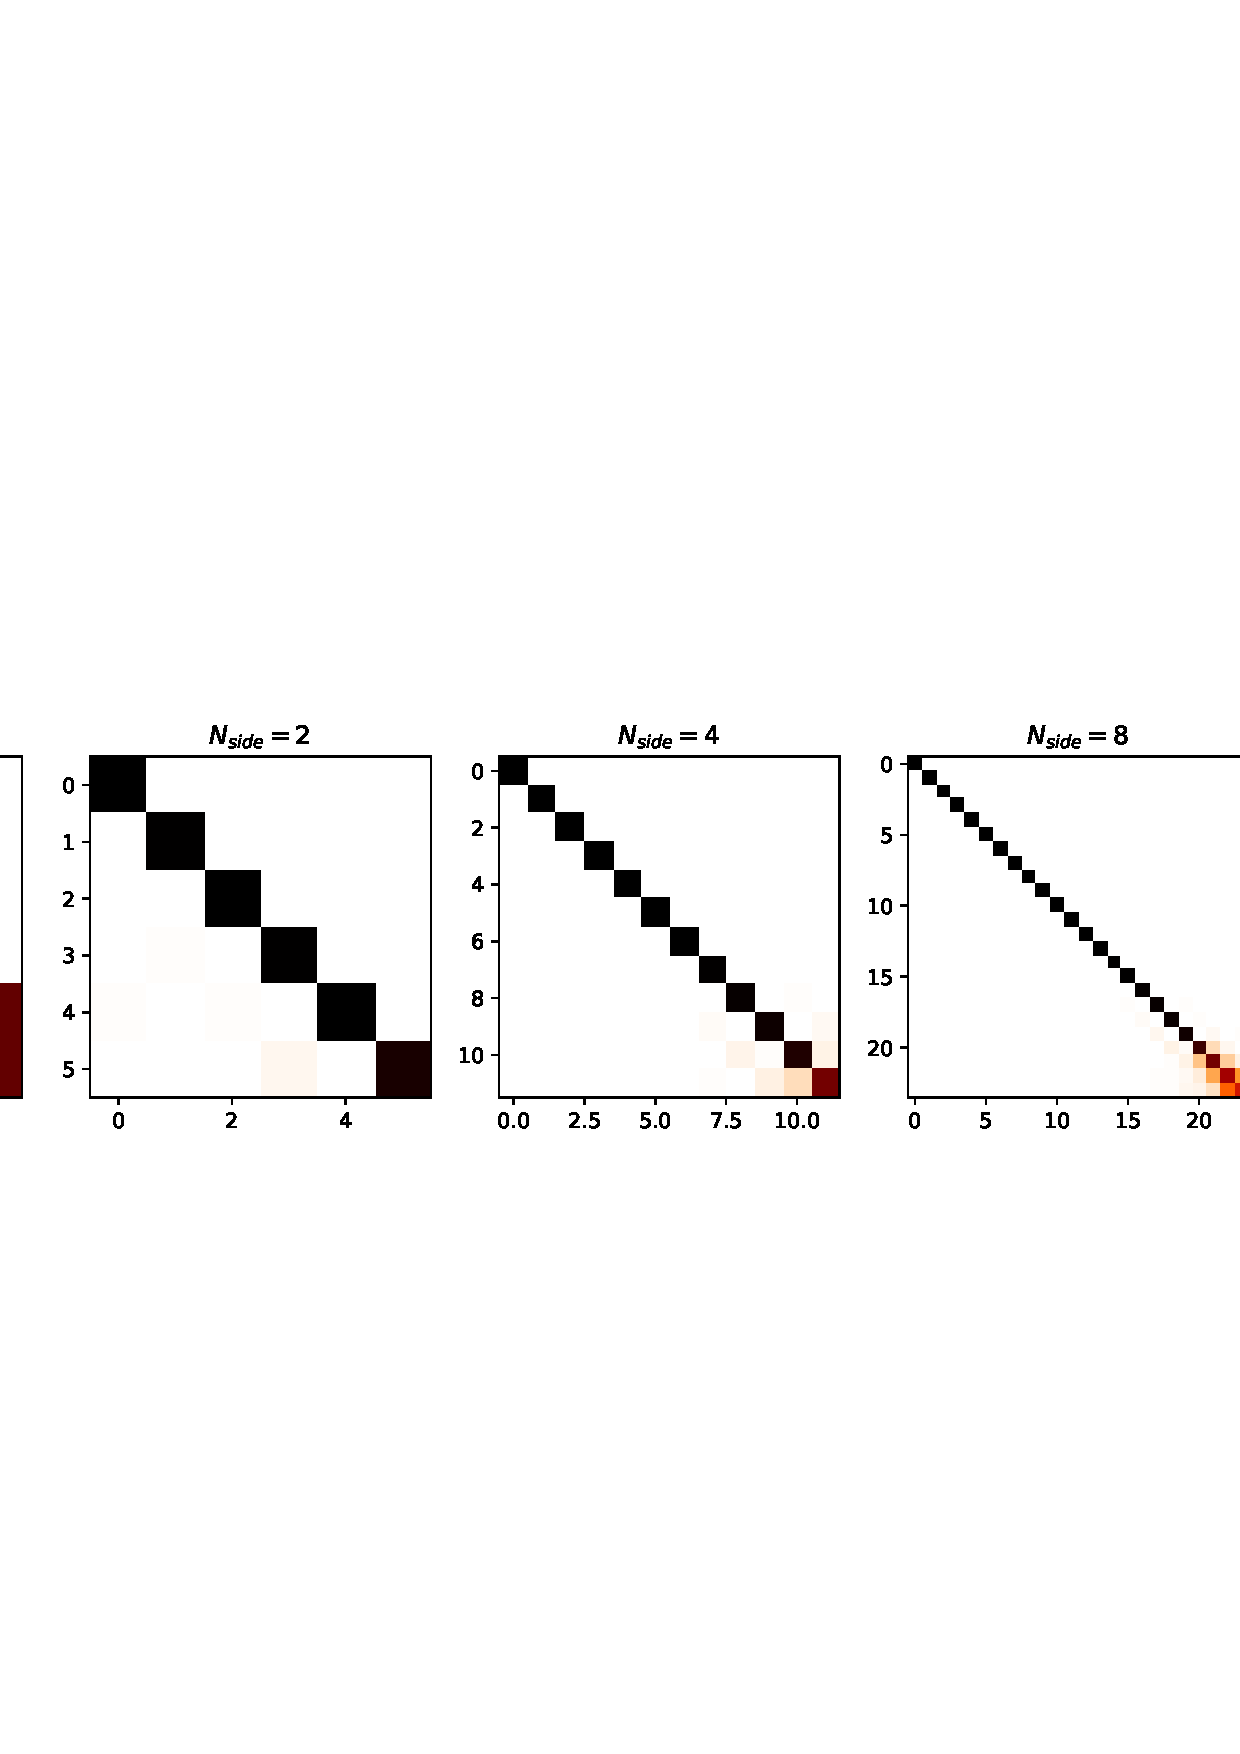
\includegraphics[width=0.9\textwidth]{../codes/02.HeatKernelGraphLaplacian/HEALPix/06_figures/deepsphere_thresholded.png}	
	\includegraphics[width=0.9\textwidth]{../codes/02.HeatKernelGraphLaplacian/HEALPix/06_figures/deepsphere_thresholded_diagonal.png}	
\end{figure}

We see that to keep the threshold fixed we need to increase the number of neighbors as $N_{side}$ gets bigger. Again, the intuition is the following: to have spectral convergence (a strong type of convergence) we need more and more global information and more precise. 
\subsection{Experimental validation}
Here we report Frederick's results with the two different constructions
